%%%%%%%%%%%%%%%%%%%%%%%%%%%%%%%%%%
The identification of the jets consisting of $b-$hadrons is performed using $b-$tagging algorithms. The performance of these $b-$tagging algorithms completely rely on identifying jets containing $b-$hadrons known as $b-$jets, $c-$hadrons known as $c-$jets and $l-$jets containing none of $b-$hadrons or $c-$hadrons. The MC estimates the probabilities of jets meeting the $b-$tagging algorithm requirements. However due to imperfections in the simulation, it is necessary to measure the (mis)tagging efficiency in data. The disagreement between data and MC increases for lower $p_T$ to higher $p_T$ jets. The simulation-to-data scale factor measured accurately for highest $p_T$ bin is extrapolated for jets with $p_T$ greater than meausred highest $p_T$. This extrapolation uncertainty needs to be taken into account for $b-$jets, $c-$jets and $l-$jets.\\
The following shows Flavor-tagging (FTAG) high $p_T$ extrapolation uncertainty red/blue plots for largest background TTB and signal masspoint 1000 $GeV$ in $1L$ channel.


\begin{figure}[htbp!]
        \begin{center} \setlength{\tabcolsep}{2.5pt}\footnotesize
        \begin{tabular}{cccc}
        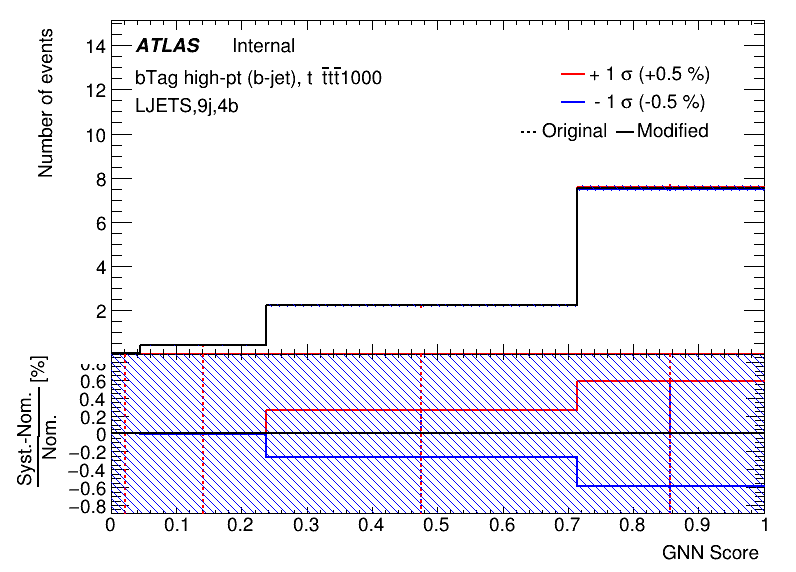
\includegraphics[width=0.23 \textwidth]{figures/red_blue_plots/FTAG_High_Pt_bjet/ljets_9j4b_BSMtttt_1000_FTAG_High_Pt_bjet.png} &
        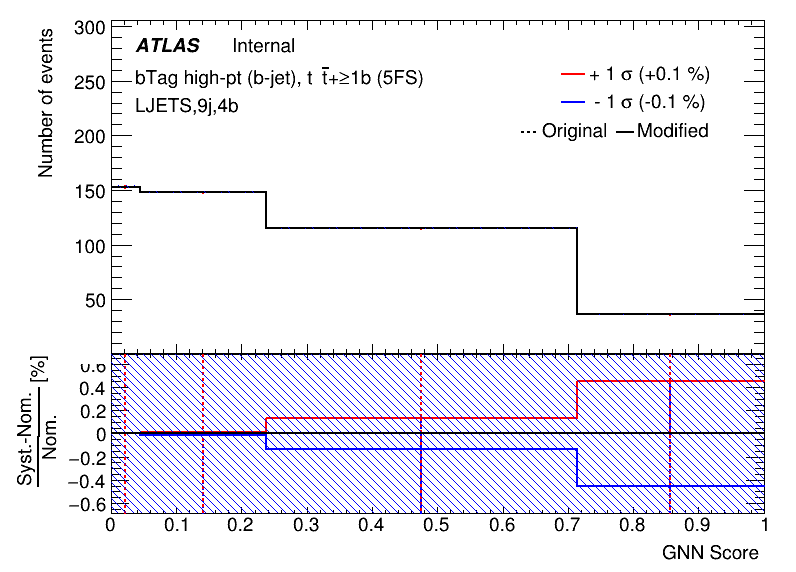
\includegraphics[width=0.23 \textwidth]{figures/red_blue_plots/FTAG_High_Pt_bjet/ljets_9j4b_TTB_FTAG_High_Pt_bjet.png} &
        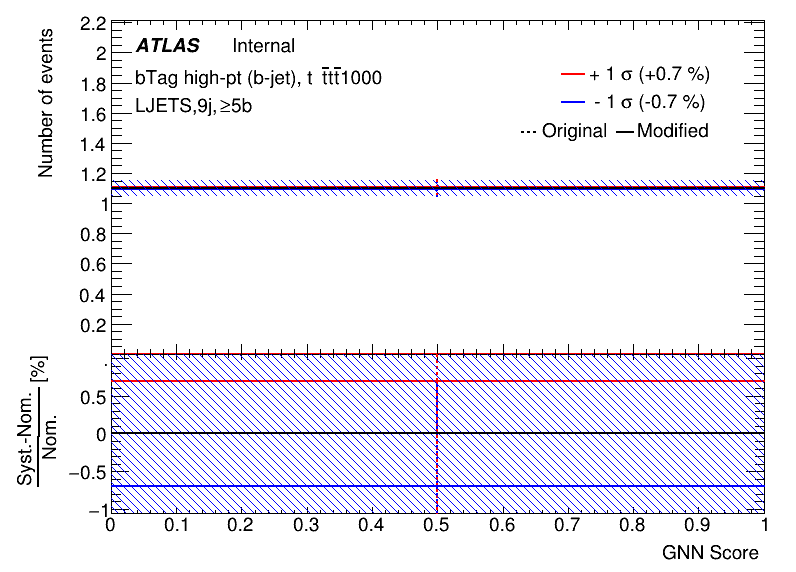
\includegraphics[width=0.23 \textwidth]{figures/red_blue_plots/FTAG_High_Pt_bjet/ljets_9jge5b_BSMtttt_1000_FTAG_High_Pt_bjet.png} &
        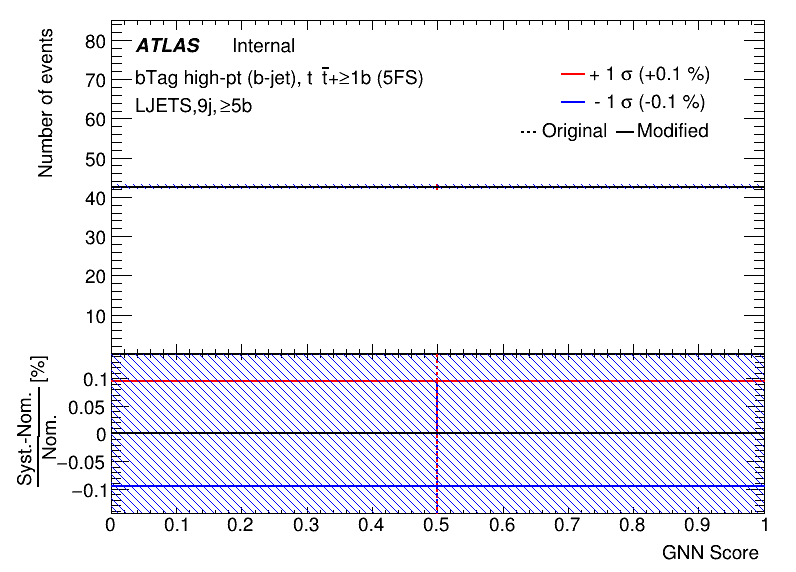
\includegraphics[width=0.23 \textwidth]{figures/red_blue_plots/FTAG_High_Pt_bjet/ljets_9jge5b_TTB_FTAG_High_Pt_bjet.png}\\

        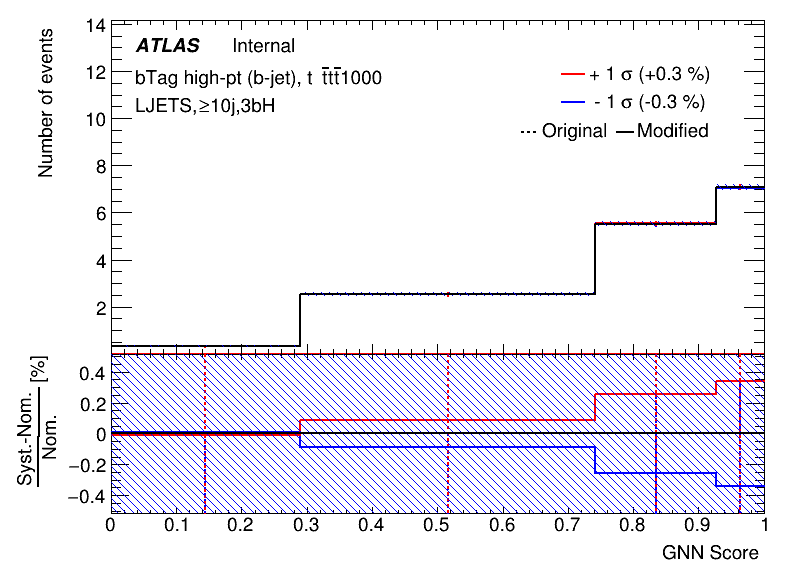
\includegraphics[width=0.23 \textwidth]{figures/red_blue_plots/FTAG_High_Pt_bjet/ljets_ge10j3bH_BSMtttt_1000_FTAG_High_Pt_bjet.png} &
        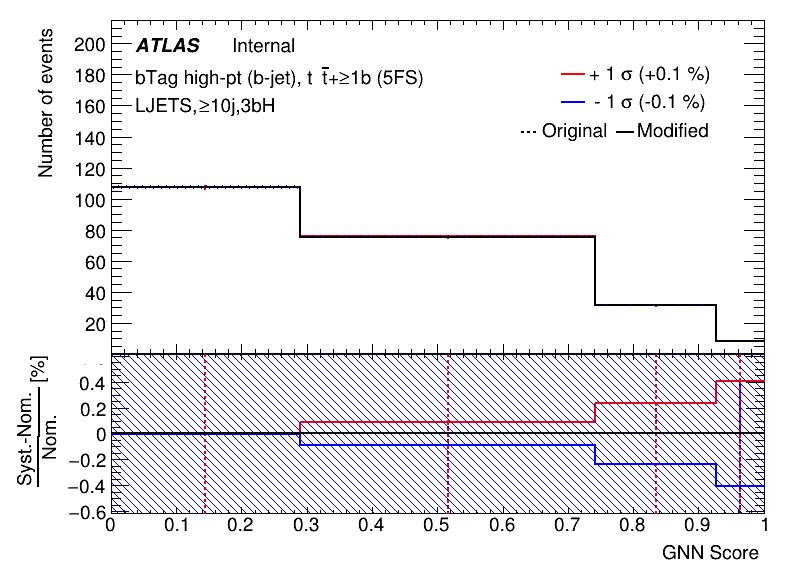
\includegraphics[width=0.23 \textwidth]{figures/red_blue_plots/FTAG_High_Pt_bjet/ljets_ge10j3bH_TTB_FTAG_High_Pt_bjet.png} &
        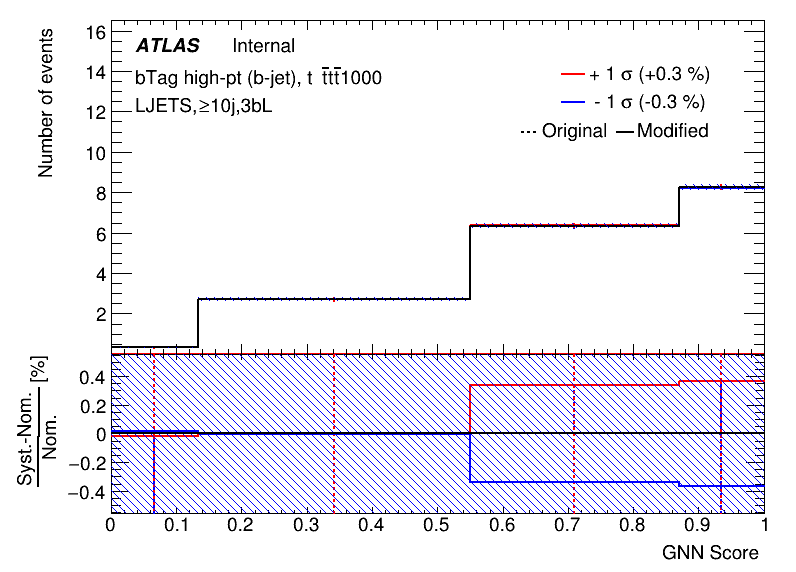
\includegraphics[width=0.23 \textwidth]{figures/red_blue_plots/FTAG_High_Pt_bjet/ljets_ge10j3bL_BSMtttt_1000_FTAG_High_Pt_bjet.png} &
        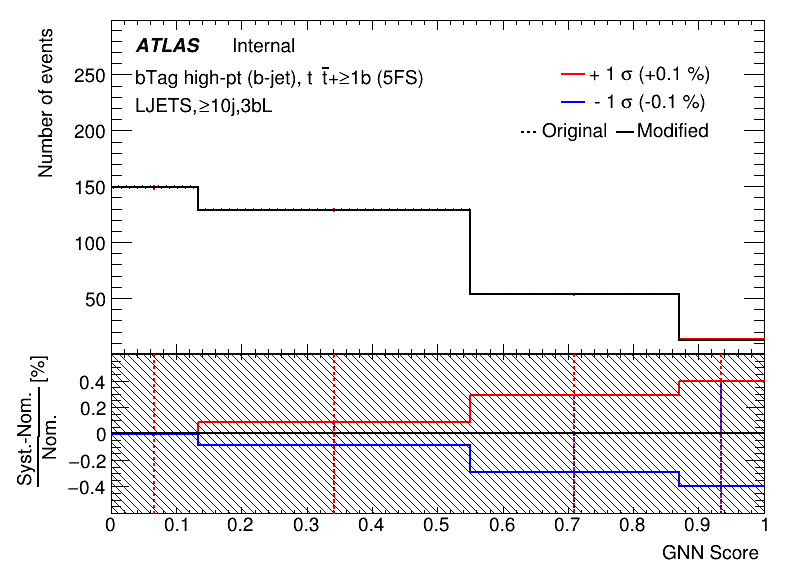
\includegraphics[width=0.23 \textwidth]{figures/red_blue_plots/FTAG_High_Pt_bjet/ljets_ge10j3bL_TTB_FTAG_High_Pt_bjet.png} \\

        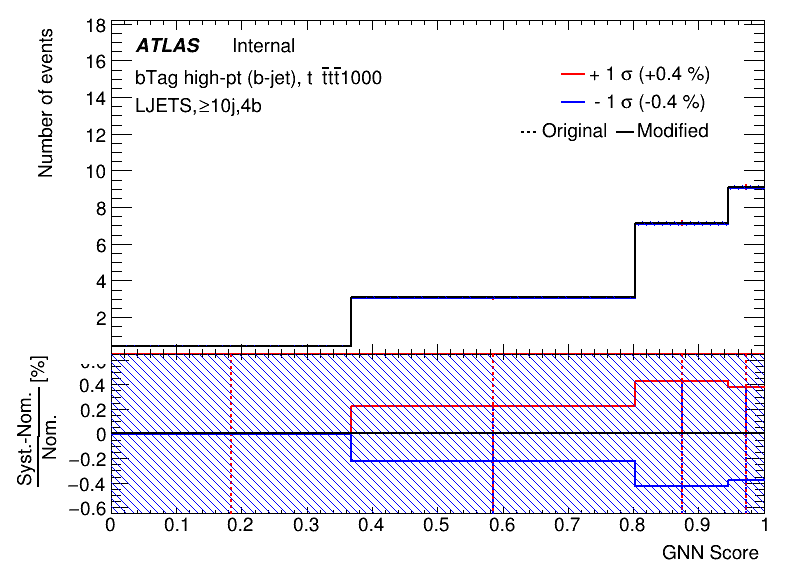
\includegraphics[width=0.23 \textwidth]{figures/red_blue_plots/FTAG_High_Pt_bjet/ljets_ge10j4b_BSMtttt_1000_FTAG_High_Pt_bjet.png} &
        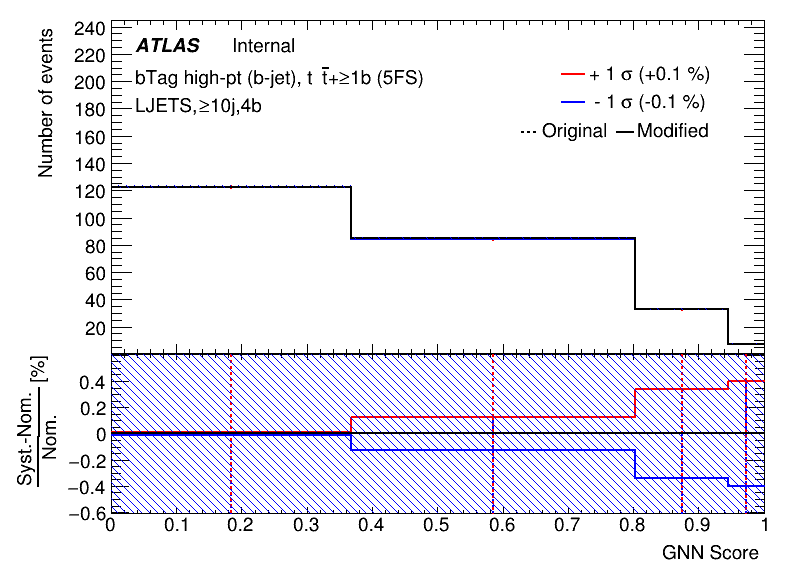
\includegraphics[width=0.23 \textwidth]{figures/red_blue_plots/FTAG_High_Pt_bjet/ljets_ge10j4b_TTB_FTAG_High_Pt_bjet.png} &
        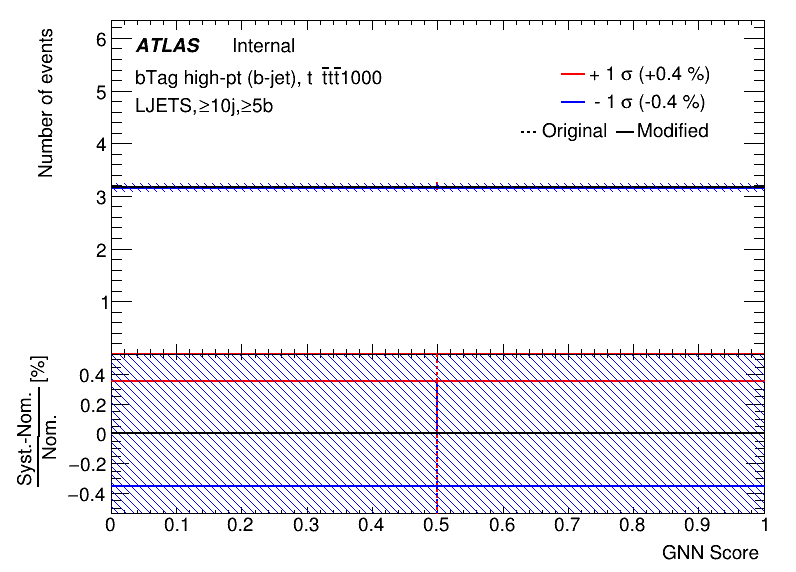
\includegraphics[width=0.23 \textwidth]{figures/red_blue_plots/FTAG_High_Pt_bjet/ljets_ge10jge5b_BSMtttt_1000_FTAG_High_Pt_bjet.png} &
        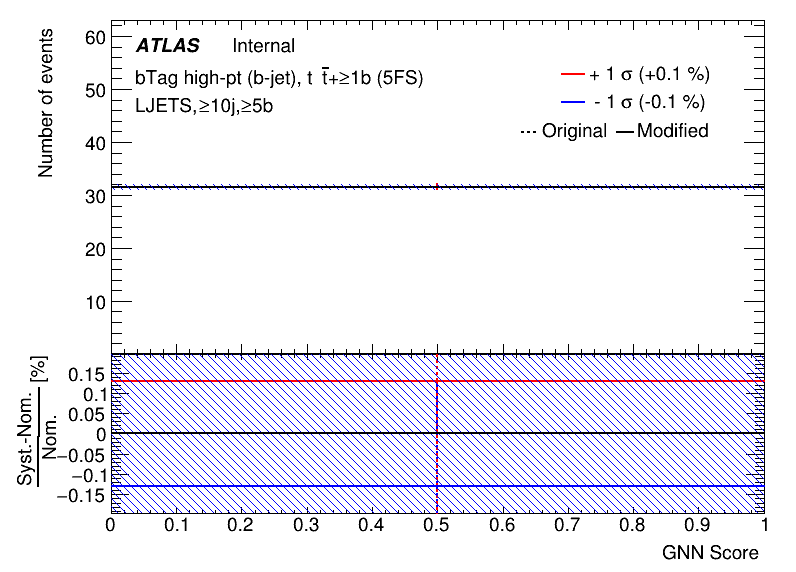
\includegraphics[width=0.23 \textwidth]{figures/red_blue_plots/FTAG_High_Pt_bjet/ljets_ge10jge5b_TTB_FTAG_High_Pt_bjet.png} \\
        \end{tabular}
        \caption{\label{fig:FTAG_highPt_bjet_1L}The figure shows red/blue plots for FTAG High $p_T$ extrapolation uncertainty for $b-$jets for TTB sample and signal masspoint 1000 $GeV$ in 1L channel.}
\end{center}
\end{figure}


\begin{figure}[htbp!]
        \begin{center} \setlength{\tabcolsep}{2.5pt}\footnotesize
        \begin{tabular}{cccc}
        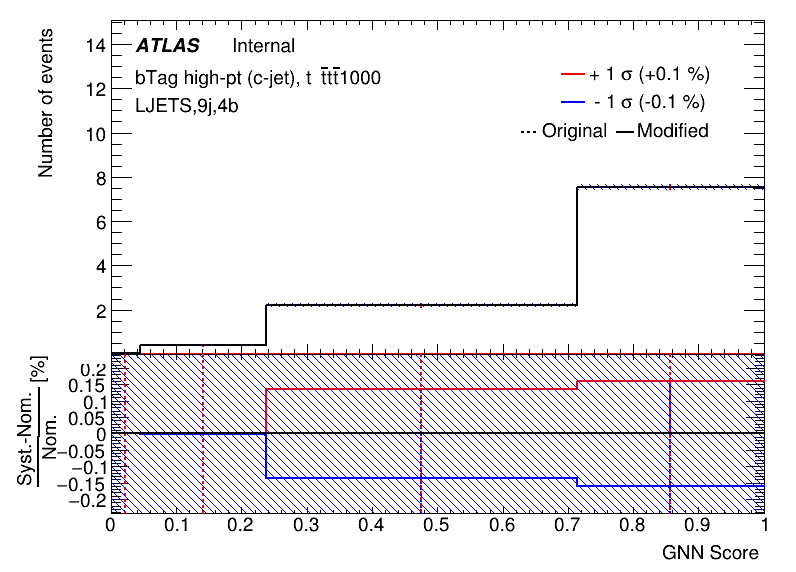
\includegraphics[width=0.23 \textwidth]{figures/red_blue_plots/FTAG_High_Pt_cjet/ljets_9j4b_BSMtttt_1000_FTAG_High_Pt_cjet.png} &
        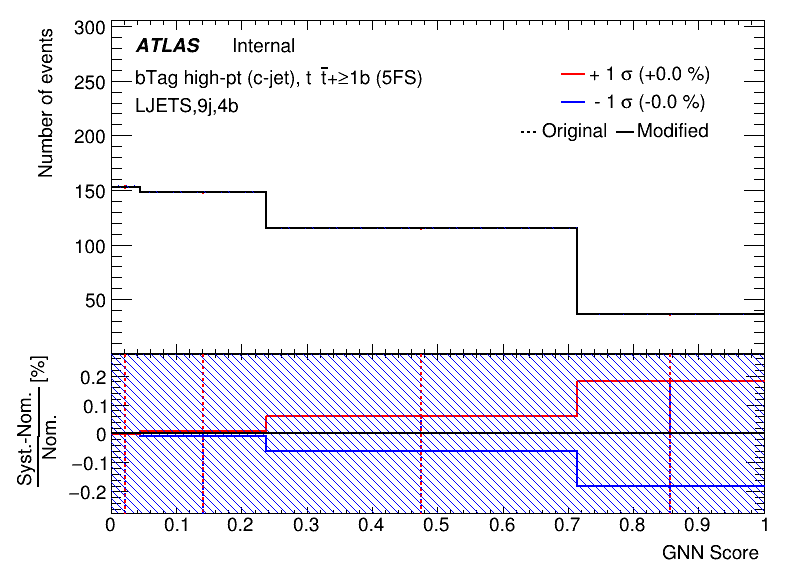
\includegraphics[width=0.23 \textwidth]{figures/red_blue_plots/FTAG_High_Pt_cjet/ljets_9j4b_TTB_FTAG_High_Pt_cjet.png} &
        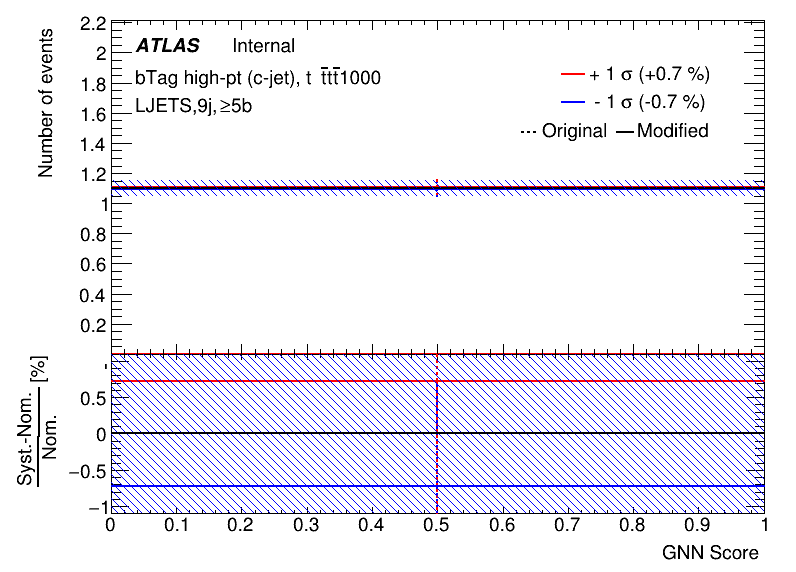
\includegraphics[width=0.23 \textwidth]{figures/red_blue_plots/FTAG_High_Pt_cjet/ljets_9jge5b_BSMtttt_1000_FTAG_High_Pt_cjet.png} &
        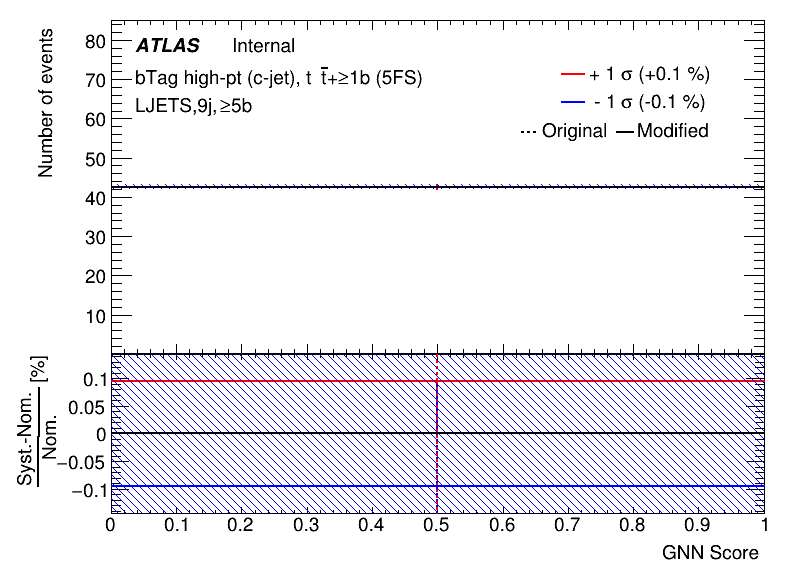
\includegraphics[width=0.23 \textwidth]{figures/red_blue_plots/FTAG_High_Pt_cjet/ljets_9jge5b_TTB_FTAG_High_Pt_cjet.png} \\

        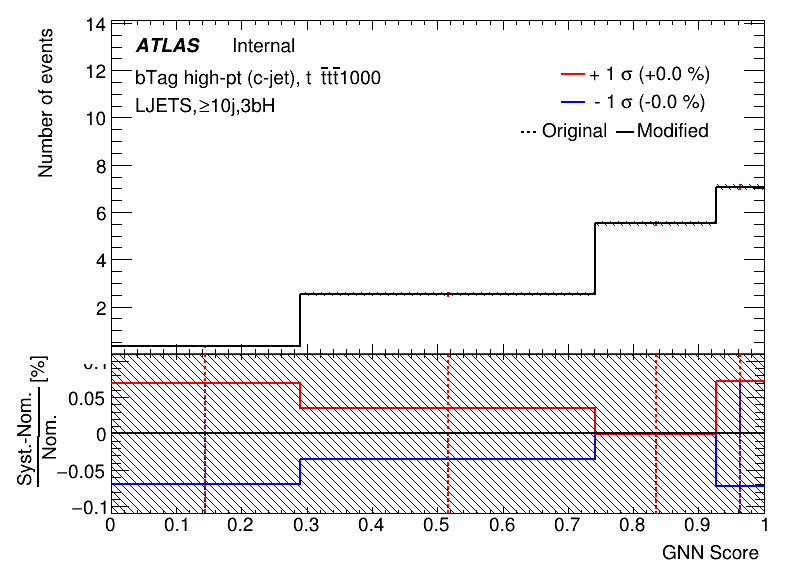
\includegraphics[width=0.23 \textwidth]{figures/red_blue_plots/FTAG_High_Pt_cjet/ljets_ge10j3bH_BSMtttt_1000_FTAG_High_Pt_cjet.png} &
        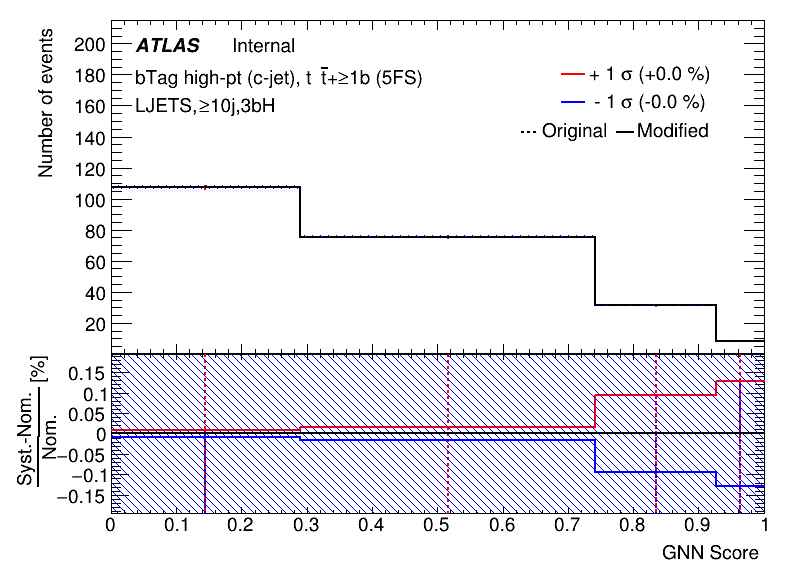
\includegraphics[width=0.23 \textwidth]{figures/red_blue_plots/FTAG_High_Pt_cjet/ljets_ge10j3bH_TTB_FTAG_High_Pt_cjet.png} &
        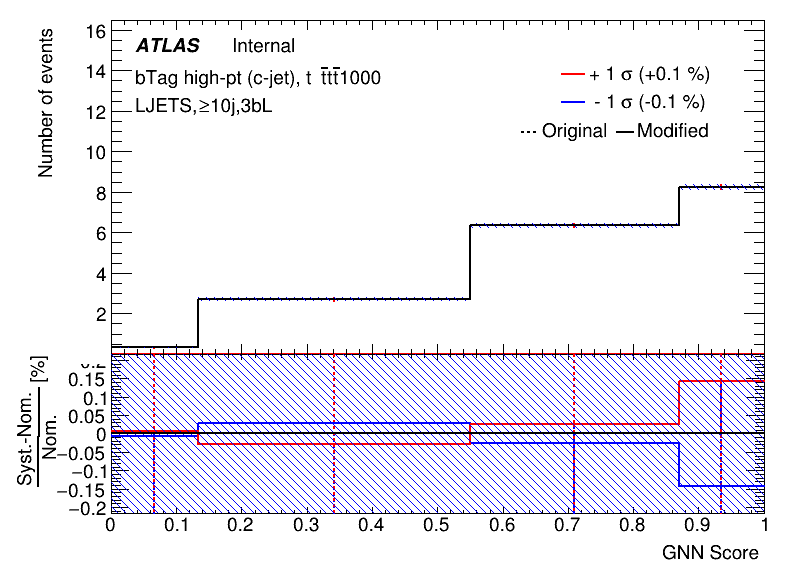
\includegraphics[width=0.23 \textwidth]{figures/red_blue_plots/FTAG_High_Pt_cjet/ljets_ge10j3bL_BSMtttt_1000_FTAG_High_Pt_cjet.png} &
        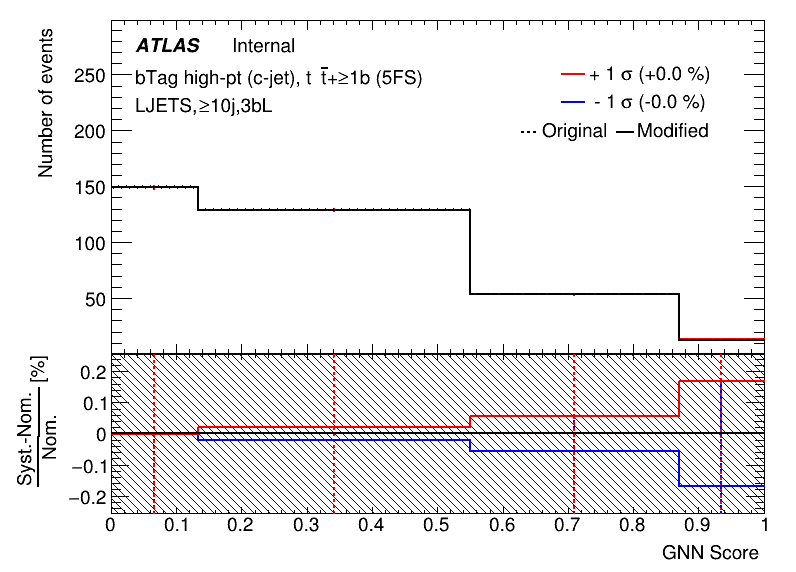
\includegraphics[width=0.23 \textwidth]{figures/red_blue_plots/FTAG_High_Pt_cjet/ljets_ge10j3bL_TTB_FTAG_High_Pt_cjet.png} \\

        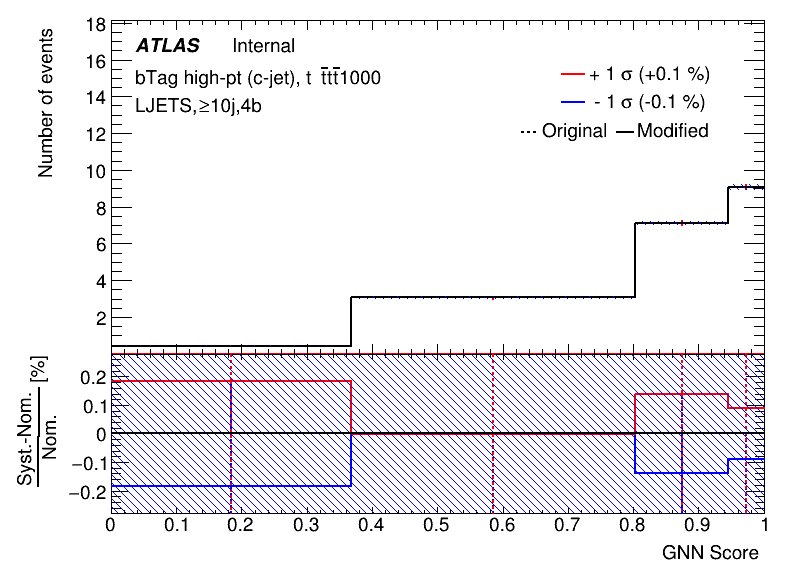
\includegraphics[width=0.23 \textwidth]{figures/red_blue_plots/FTAG_High_Pt_cjet/ljets_ge10j4b_BSMtttt_1000_FTAG_High_Pt_cjet.png} &
        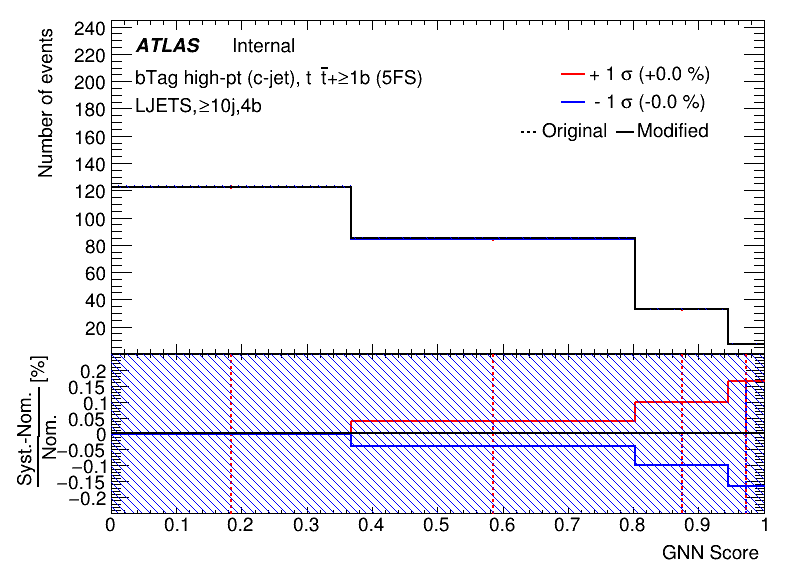
\includegraphics[width=0.23 \textwidth]{figures/red_blue_plots/FTAG_High_Pt_cjet/ljets_ge10j4b_TTB_FTAG_High_Pt_cjet.png} &
        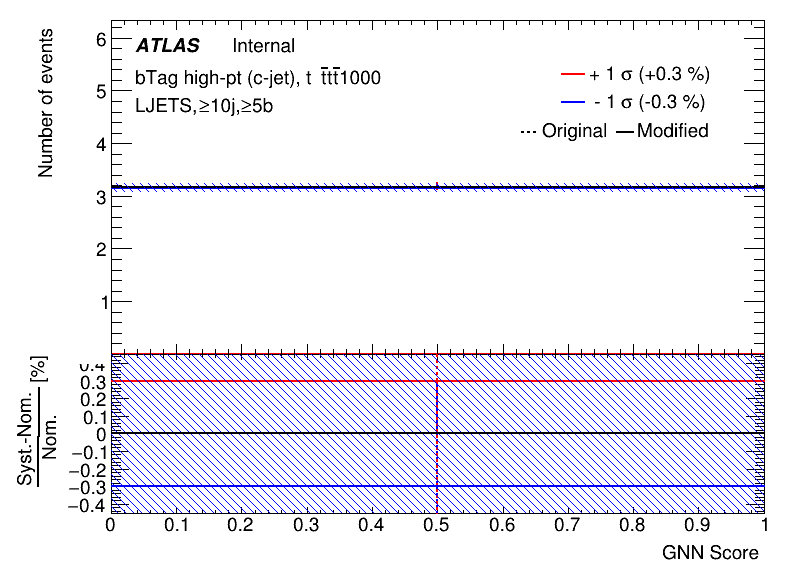
\includegraphics[width=0.23 \textwidth]{figures/red_blue_plots/FTAG_High_Pt_cjet/ljets_ge10jge5b_BSMtttt_1000_FTAG_High_Pt_cjet.png} &
        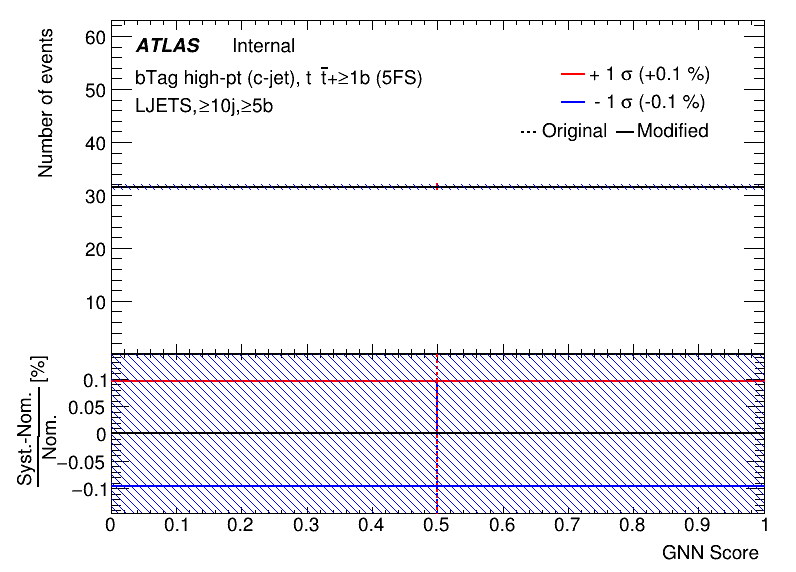
\includegraphics[width=0.23 \textwidth]{figures/red_blue_plots/FTAG_High_Pt_cjet/ljets_ge10jge5b_TTB_FTAG_High_Pt_cjet.png} \\
        \end{tabular}
        \caption{\label{fig:FTAG_highPt_cjet_1L}The figure shows red/blue plots for FTAG High $p_T$ extrapolation uncertainty for $c-$jets for TTB sample and signal masspoint 1000 $GeV$ in 1L channel.}
\end{center}
\end{figure}


\begin{figure}[htbp!]
        \begin{center} \setlength{\tabcolsep}{2.5pt}\footnotesize
        \begin{tabular}{cccc}
        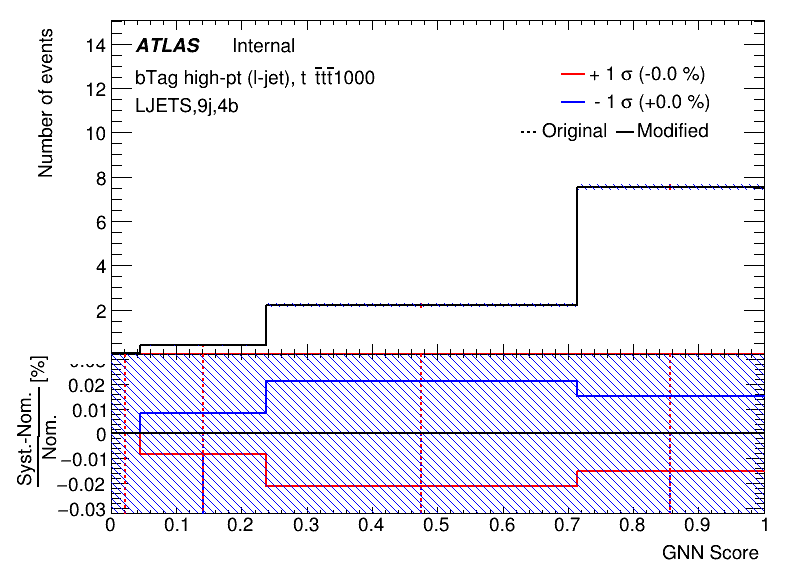
\includegraphics[width=0.23 \textwidth]{figures/red_blue_plots/FTAG_High_Pt_ljet/ljets_9j4b_BSMtttt_1000_FTAG_High_Pt_ljet.png} &
        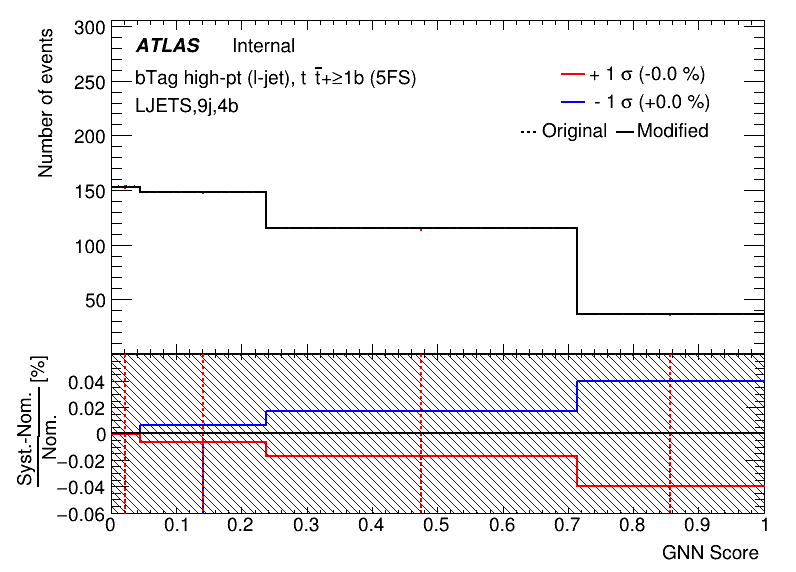
\includegraphics[width=0.23 \textwidth]{figures/red_blue_plots/FTAG_High_Pt_ljet/ljets_9j4b_TTB_FTAG_High_Pt_ljet.png} &
        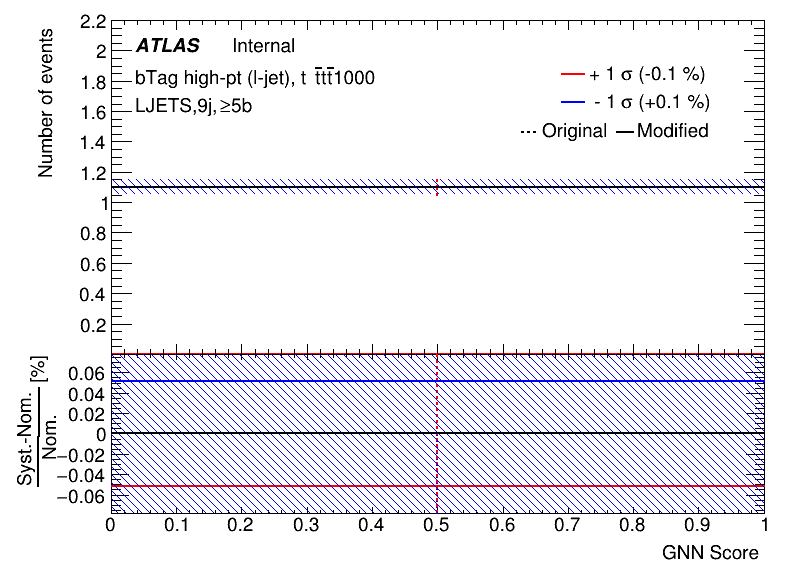
\includegraphics[width=0.23 \textwidth]{figures/red_blue_plots/FTAG_High_Pt_ljet/ljets_9jge5b_BSMtttt_1000_FTAG_High_Pt_ljet.png} &
        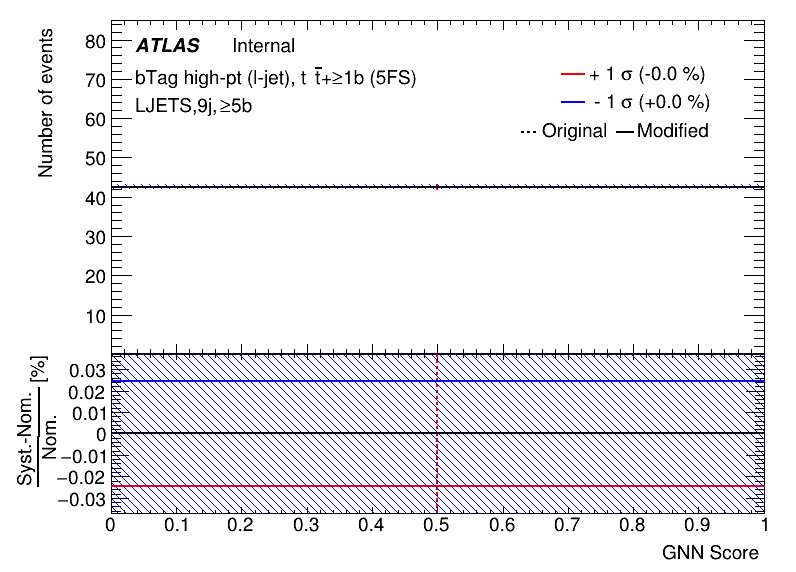
\includegraphics[width=0.23 \textwidth]{figures/red_blue_plots/FTAG_High_Pt_ljet/ljets_9jge5b_TTB_FTAG_High_Pt_ljet.png} \\

        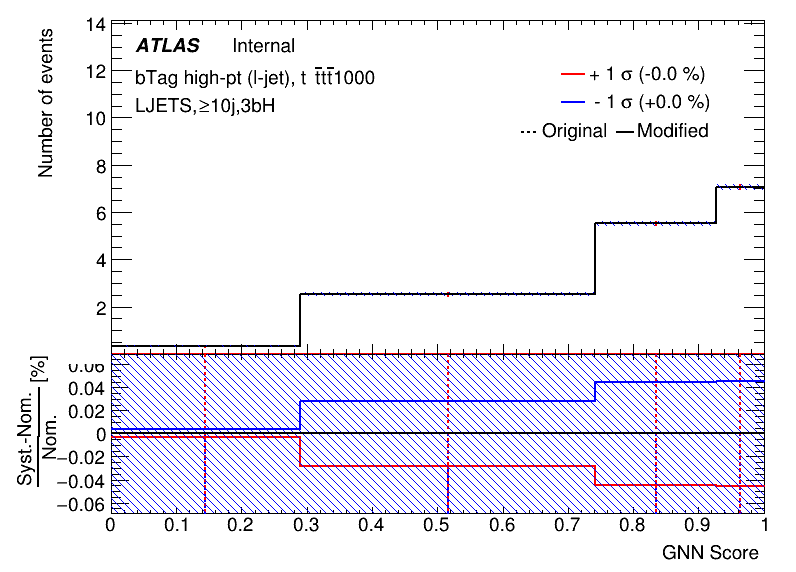
\includegraphics[width=0.23 \textwidth]{figures/red_blue_plots/FTAG_High_Pt_ljet/ljets_ge10j3bH_BSMtttt_1000_FTAG_High_Pt_ljet.png} &
        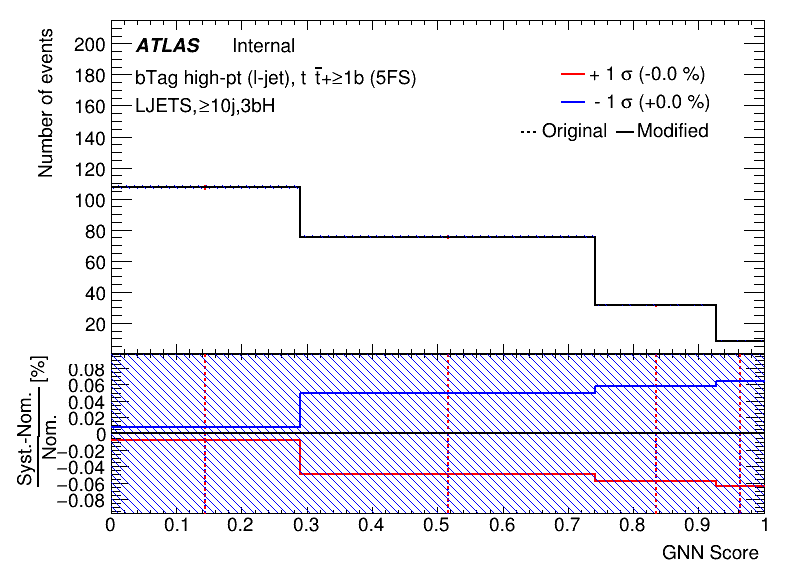
\includegraphics[width=0.23 \textwidth]{figures/red_blue_plots/FTAG_High_Pt_ljet/ljets_ge10j3bH_TTB_FTAG_High_Pt_ljet.png} &
        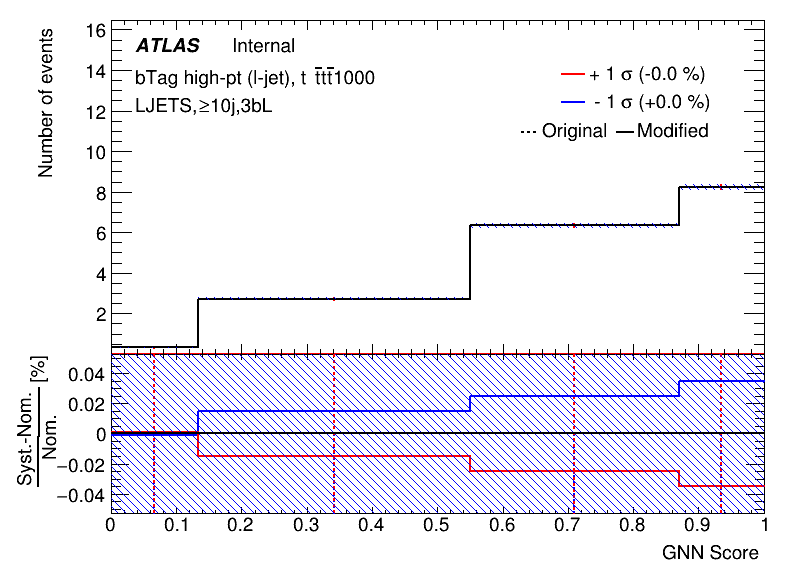
\includegraphics[width=0.23 \textwidth]{figures/red_blue_plots/FTAG_High_Pt_ljet/ljets_ge10j3bL_BSMtttt_1000_FTAG_High_Pt_ljet.png} &
        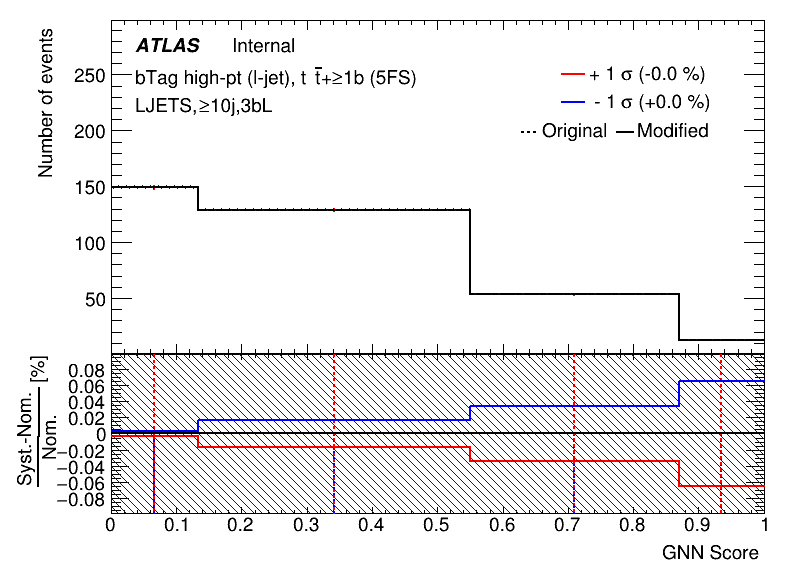
\includegraphics[width=0.23 \textwidth]{figures/red_blue_plots/FTAG_High_Pt_ljet/ljets_ge10j3bL_TTB_FTAG_High_Pt_ljet.png} \\

        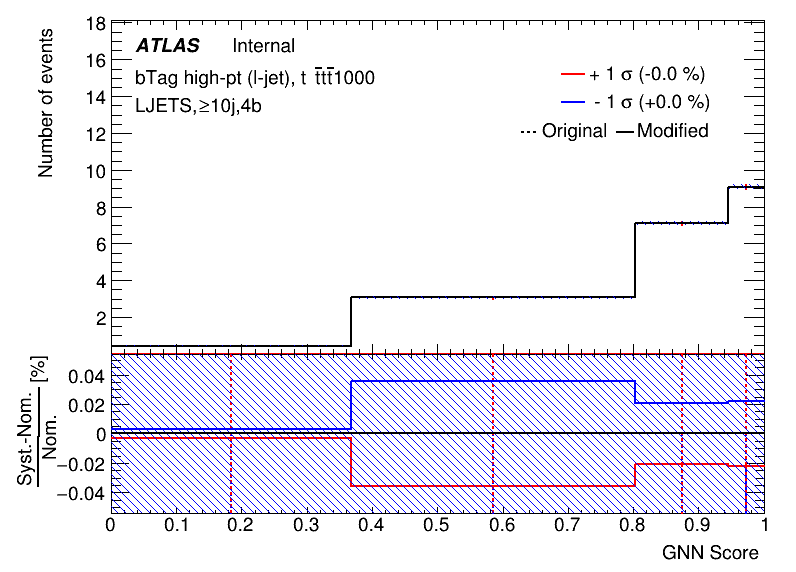
\includegraphics[width=0.23 \textwidth]{figures/red_blue_plots/FTAG_High_Pt_ljet/ljets_ge10j4b_BSMtttt_1000_FTAG_High_Pt_ljet.png} &
        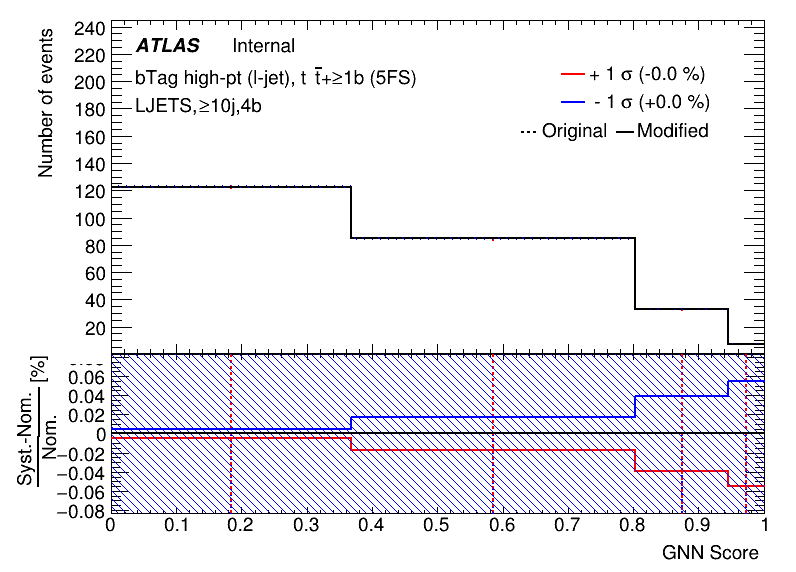
\includegraphics[width=0.23 \textwidth]{figures/red_blue_plots/FTAG_High_Pt_ljet/ljets_ge10j4b_TTB_FTAG_High_Pt_ljet.png} &
        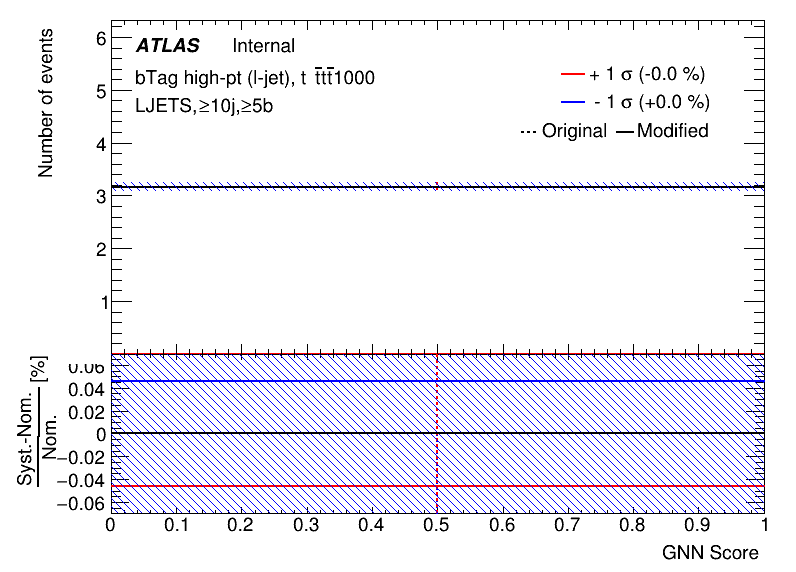
\includegraphics[width=0.23 \textwidth]{figures/red_blue_plots/FTAG_High_Pt_ljet/ljets_ge10jge5b_BSMtttt_1000_FTAG_High_Pt_ljet.png} &
        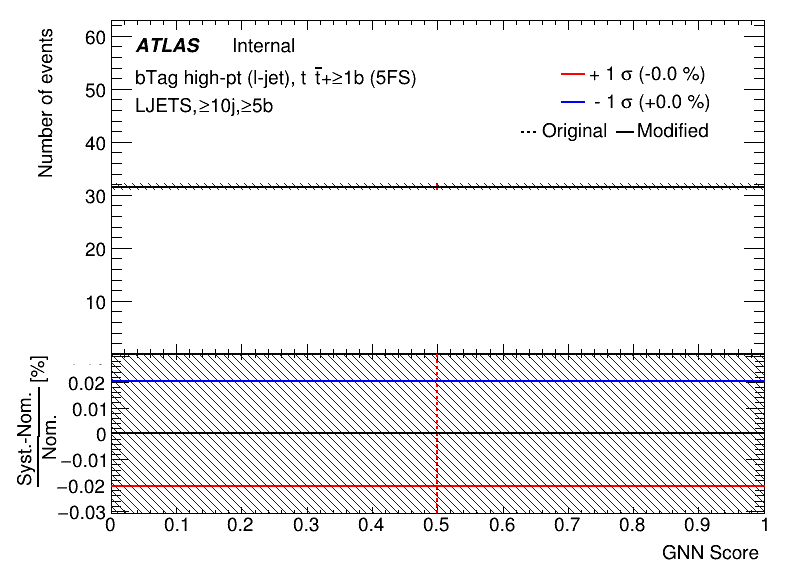
\includegraphics[width=0.23 \textwidth]{figures/red_blue_plots/FTAG_High_Pt_ljet/ljets_ge10jge5b_TTB_FTAG_High_Pt_ljet.png} \\
        \end{tabular}
        \caption{\label{fig:FTAG_highPt_ljet_1L}The figure shows red/blue plots for FTAG High $p_T$ extrapolation uncertainty for $l-$jets for TTB sample and signal masspoint 1000 $GeV$ in 1L channel.}
\end{center}
\end{figure}


